\section{Criptografia e assinatura digital}

\subsection{Criptografia}
\begin{frame}
\frametitle{Criptografia}

\begin{itemize}
\item estenografia (escrita oculta) - ocultar uma mensagem dentro de outra
\item criptografia (escrita segura)
\end{itemize}

\end{frame}



\begin{frame}[allowframebreaks]
\frametitle{Estenografia}
\begin{figure}[h]
\centering
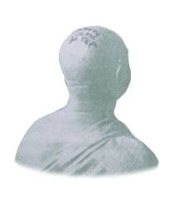
\includegraphics[width=0.33\textwidth,height=0.7\textheight,keepaspectratio]{figures/herodotus.jpg}
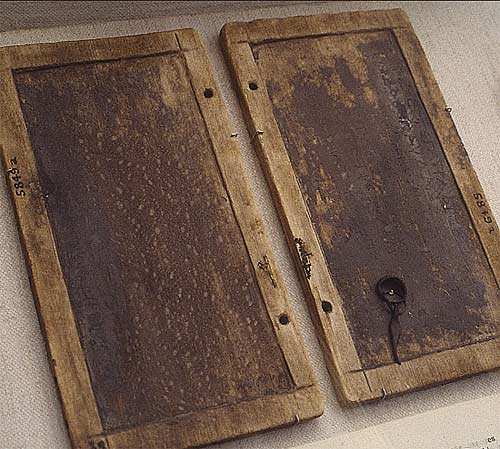
\includegraphics[width=0.33\textwidth,height=0.7\textheight,keepaspectratio]{figures/waxtablet.jpg}
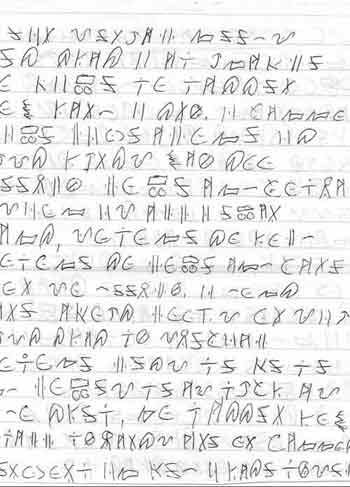
\includegraphics[width=0.33\textwidth,height=0.7\textheight,keepaspectratio]{figures/gangcode.jpg}
\caption{Tatuagem de Heródoto. Tábuas de cera. Código de gangues.}
\label{fig-estenografia}
\end{figure}

\begin{itemize}
\item tinta invisível
\item micropontos
\item bits de menor valor
\end{itemize}
\end{frame}




\begin{frame}
\frametitle{Cifra de transposição}

A Cítala é um ferramenta de criptografia utilizada pelos gregos antigos e espartanos para envio de mensagens secretas
durante as campanhas militares.
\begin{figure}[h]
\centering
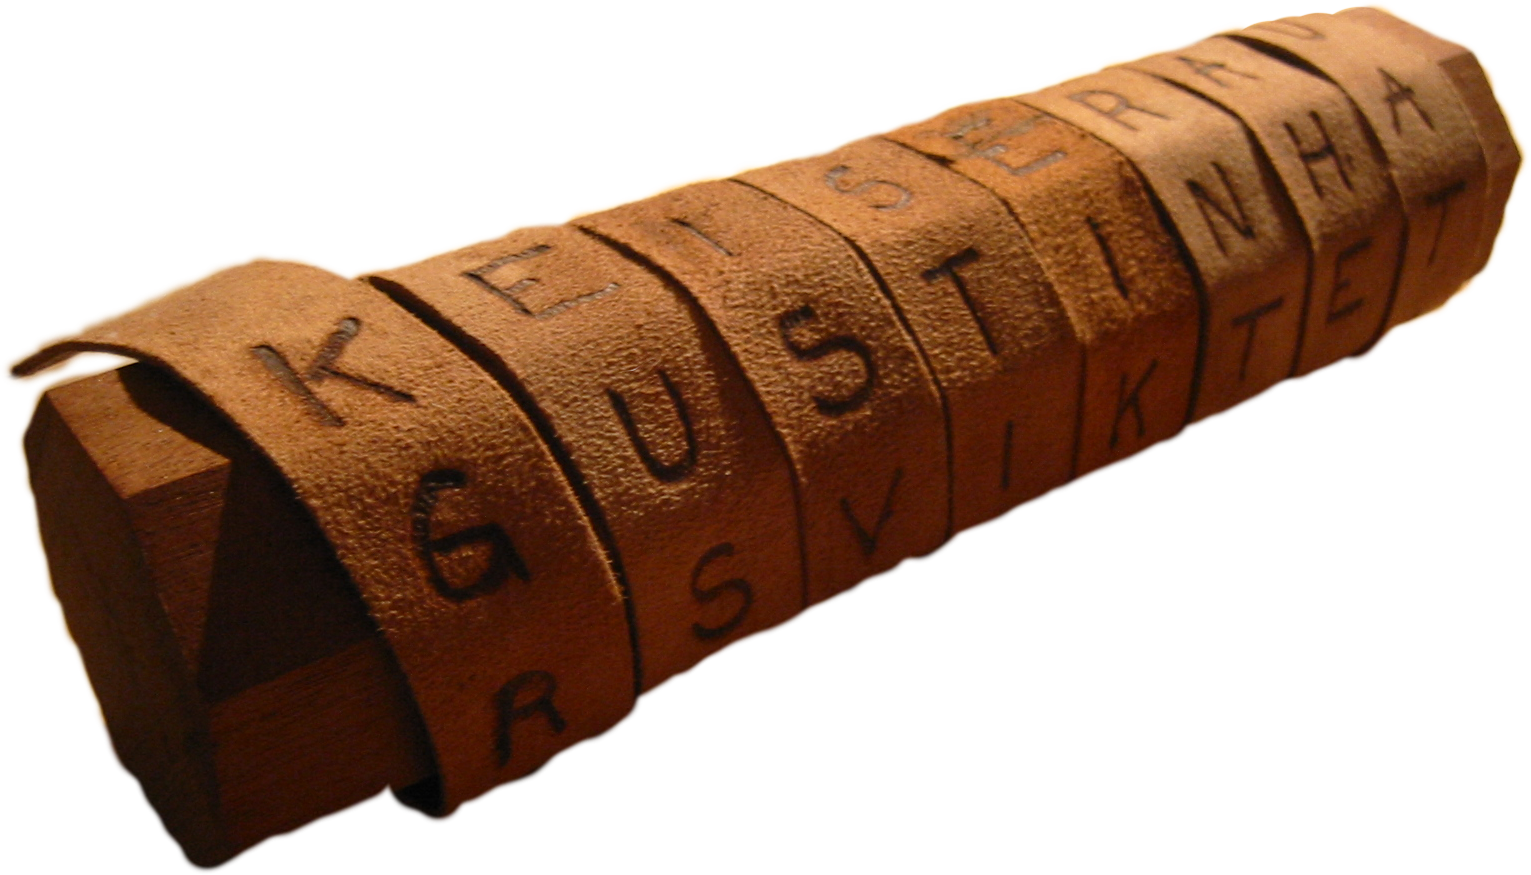
\includegraphics[width=0.6\textwidth,height=0.5\textheight,keepaspectratio]{figures/cifratransposicao.png}
\caption{Cítala (ou bastão de Licurgo). Cifra de transposição. \url{https://en.wikipedia.org/wiki/Scytale}}
\label{fig-cifratrans}
\end{figure}
\end{frame}


\begin{frame}[allowframebreaks]
\frametitle{Cifra de César}

\begin{figure}[h]
\centering
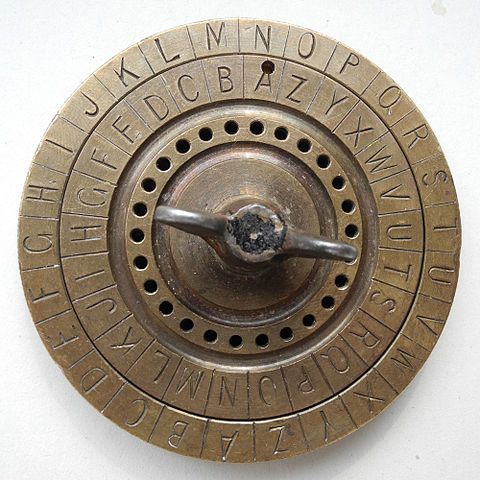
\includegraphics[width=0.5\textwidth,height=0.5\textheight,keepaspectratio]{figures/caesar.jpg}
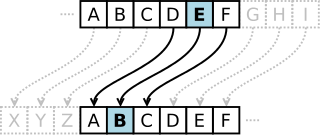
\includegraphics[width=0.5\textwidth,height=0.5\textheight,keepaspectratio]{figures/CaesarCipher.png}
\caption{Cifra de César. \url{https://en.wikipedia.org/wiki/Caesar_cipher}}
\label{fig-cifracaesar}
\end{figure}

ROT13 (\emph{rotate by 13 places}) é um caso específico da cifra de César com deslocamento de 13 posições, o que 
faz com que o algoritmo de codificação e decodificação seja o mesmo.
ROT13 era utilizado na década de 80 para esconder piadas potencialmente ofensivas, respostas de enigmas, ou 
outros \emph{spoilers}. É utilizado para esconder endereços de e-mails de \emph{spam bots}.
\url{https://en.wikipedia.org/wiki/ROT13}

\framebreak

\begin{figure}[h]
\centering
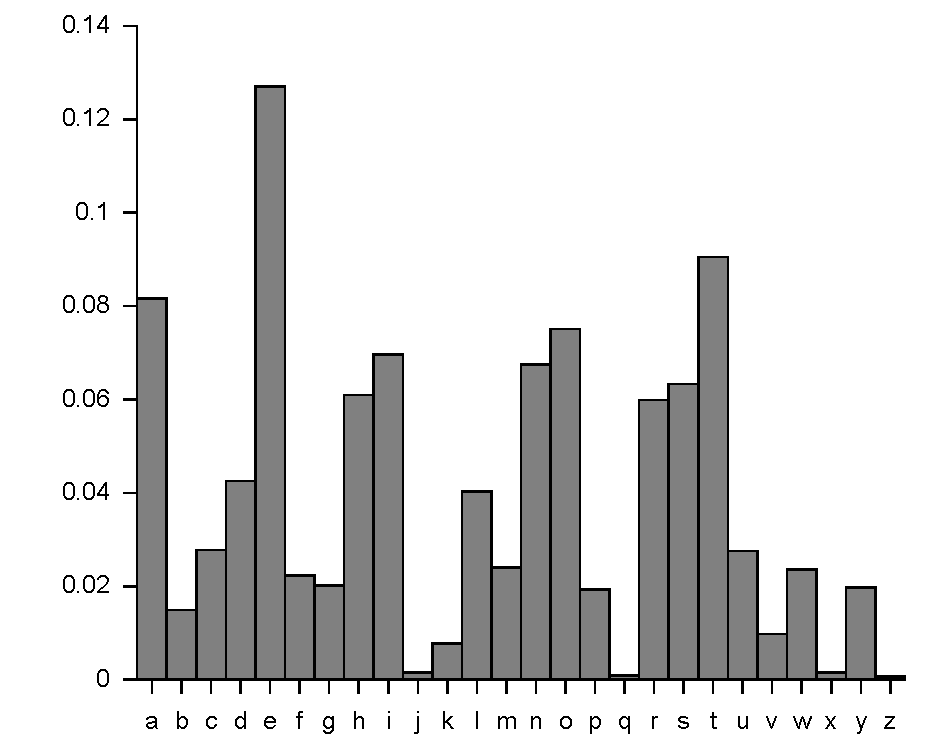
\includegraphics[width=0.5\textwidth,height=0.5\textheight,keepaspectratio]{figures/English_letter_frequency.pdf}
\caption{Distribuição de frequência dos caracteres no Inglês. \url{https://en.wikipedia.org/wiki/Caesar_cipher}}
\label{fig-eng-letters-dist}
\end{figure}

\end{frame}



\begin{frame}
\frametitle{Cifra de Beale}
Substitui cada palavra ou sequência por um código (utilizando uma referência, por exemplo, um livro).

\begin{figure}[h]
\centering
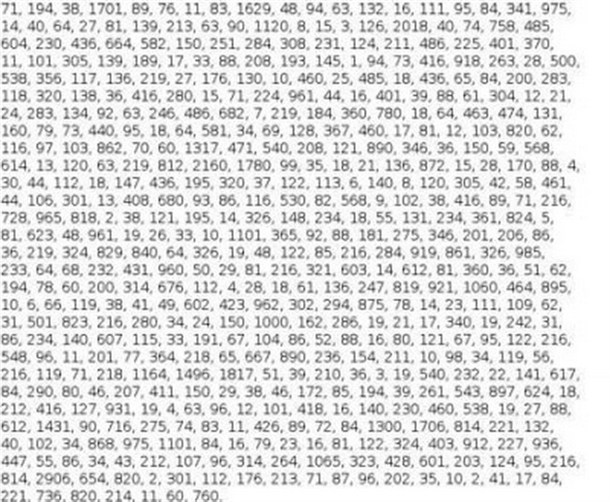
\includegraphics[width=0.7\textwidth,height=0.5\textheight,keepaspectratio]{figures/beale.jpg}
\caption{Cifra de Beale.}
\label{fig-beale}
\end{figure}

\end{frame}






\begin{frame}[allowframebreaks]
\frametitle{Zodíaco}

\begin{figure}[h]
\centering
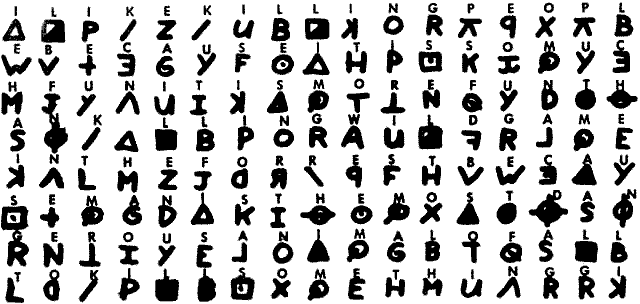
\includegraphics[width=0.5\textwidth,height=0.5\textheight,keepaspectratio]{figures/zodiaccipher.png}
\caption{Zodíaco. Múltiplos símbolos para caracteres comuns do alfabeto e anagramas.}
\label{fig-zodiac}
\end{figure}

O código foi quebrado apenas no final de 2020.\\
\fullcite{goodin_zodiac_2020}

\vspace{2ex}
\fullcite{bauer_zodiac_nodate}

\end{frame}


\begin{frame}
\frametitle{Vigenère Cipher}

Cifra polialfabética (cifra baseada na substituição, usando vários alfabetos de substituição).
Utiliza as letras da chave para selecionar a coluna e as letras da mensagem para selecionar a linha.

\begin{figure}[h]
\centering
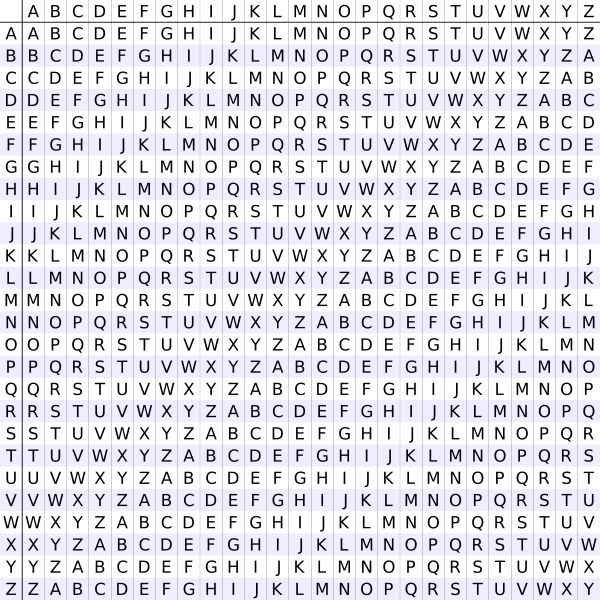
\includegraphics[width=0.8\textwidth,height=0.7\textheight,keepaspectratio]{figures/vigenere.png}
\caption{Cifra de Vigenère. Exemplo: mensagem ATTACKATDAWN, chave LEMONLEMONLE, texto cifrado LXFOPVEFRNHR.}
\label{fig-vigenere}
\end{figure}

\end{frame}


\begin{frame}
\frametitle{Cifras polialfabéticas baseadas em rotores}
\scriptsize
\begin{figure}[h]
\centering
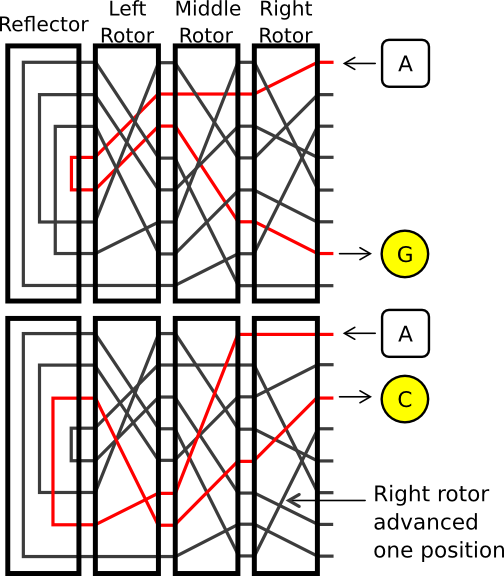
\includegraphics[width=0.5\textwidth,height=0.5\textheight,keepaspectratio]{figures/enigmaaction.png}
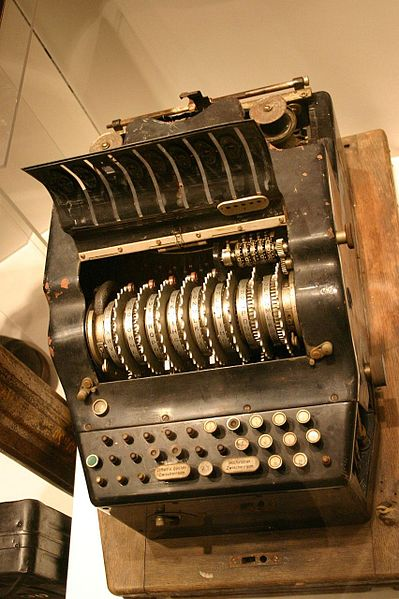
\includegraphics[width=0.5\textwidth,height=0.5\textheight,keepaspectratio]{figures/enigma.jpg}
\caption{Enigma.}
\label{fig-enigma}
\end{figure}
\vspace{-3ex}
\fullcite{cnetenigma,numberphileenigma1,numberphileenigma2}
\end{frame}



\begin{frame}
\frametitle{Princípio de Kerckhoff}
\begin{itemize}
\item Um sistema de criptografia deve ser seguro mesmo se tudo sobre ele for público, exceto a chave.
\item Não confie em segurança por obscuridade.
\end{itemize}

\vspace{2ex}
\begin{quote}
o inimigo conhece o sistema, (...) deve-se projetar sistemas sob o pressuposto de que o inimigo
irá rapidamente obter familiaridade com eles.
% "the enemy knows the system",[1] i.e., "one ought to design systems under the assumption that the enemy will immediately gain full familiarity with them".
\end{quote}

\fullcite{Shannon1949}

\end{frame}

\begin{frame}
\frametitle{Problemas da criptografia clássica}
\begin{itemize}
\item tornaram-se fracas em face da capacidade computacional dos computadores modernos
\item os métodos eram criados \emph{ad hoc}, sem existir definição e prova de segurança
\item o conhecimento de criptografia estava restrito a militares e agência de inteligência
\item o número de chaves cresce quadraticamente com o número de participantes (cada comunicação entre pares deve possuir uma chave diferente)
\end{itemize}
\end{frame}

\begin{frame}
\frametitle{Criptografia moderna}
\begin{itemize}
\item padronização das primitivas de criptografia
\item invenção da criptografia de chave pública
\item formalização da definição de segurança
\item aumento da capacidade computacional e internet
\item liberação das restrições de criptografia
\end{itemize}
\end{frame}


\begin{frame}[allowframebreaks]
\frametitle{Diffie-Hellman}
O método proposto por Whitfield Diffie e Martin Hellman permite que duas partes,
que não possuem conhecimento prévio uma da outra, troquem chaves de maneira segura através de um canal público.

\begin{figure}[h]
\centering
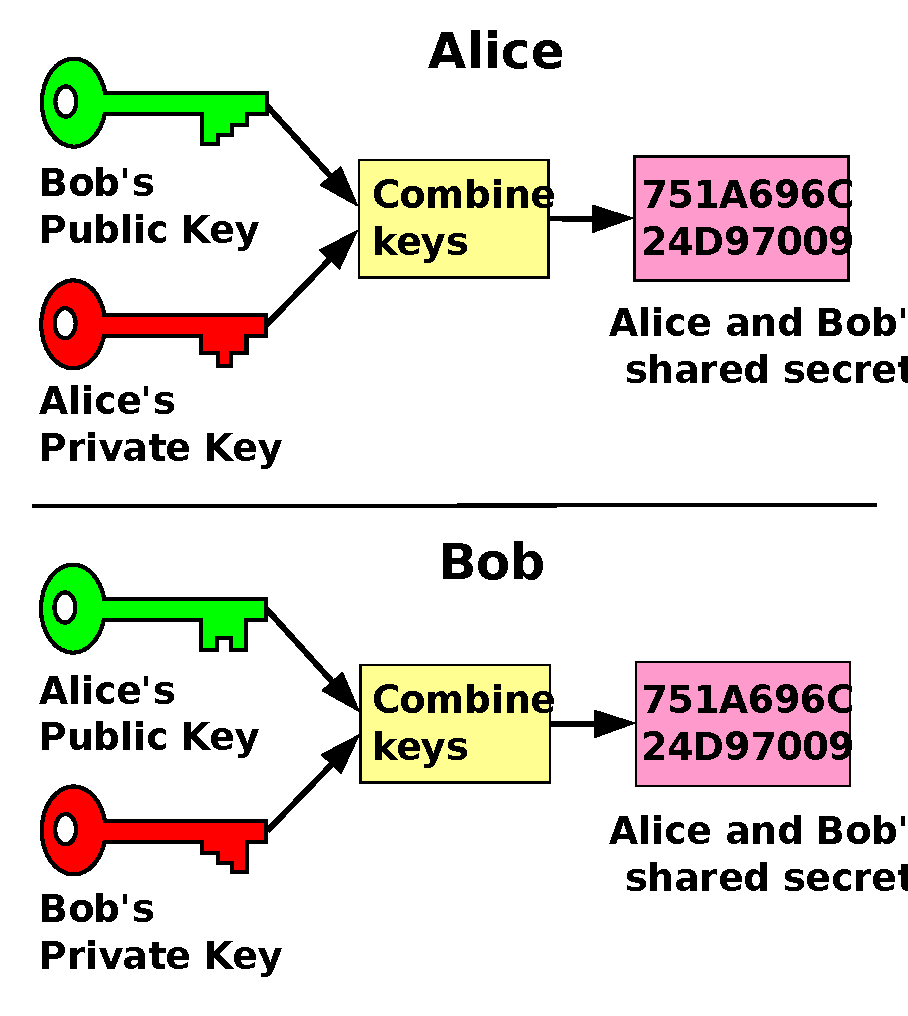
\includegraphics[width=0.5\textwidth,height=0.5\textheight,keepaspectratio]{figures/public_key_shared_secret.pdf}
\caption{Esquema de troca de chaves Diffie-Hellman.}
\label{fig-diffiehellman}
\end{figure}

\framebreak
\begin{itemize}
\item Alice seleciona um grupo $G$ (grupo matemático), um gerador $g$, e um valor aleatório $x$.
\item Alice calcula $A = g^x$ e envia para Bob ($G$,$g$,$A$).
\item Bob seleciona aleatoriamente $y$, calcula $B = g^y$, e envia $B$ para Alice.
\item Alice calcula $K = B^x= g^{(xy)}$.
\item Bob calcula $K = A^y= g^{(xy)}$.
\end{itemize}

$K$ fica sendo a chave que será utilizada na comunicação entre Alice e Bob.

Eve está escutando o canal e obtém ($G$,$g$,$A$,$B$) = ($G$,$g$,$g^x$,$g^y$).

Não existe maneira eficiente de calcular $g^{(xy)}$.

\vspace{3ex}
\url{https://www.irongeek.com/diffie-hellman.php}


\framebreak
Problemas:
\begin{itemize}
\item ataque \emph{man in the middle}
\item é necessário estabelecer $n^2$ chaves para a comunicação entre $n$ partes ou realizar este protocolo no início de cada comunicação
\item computação sobre alguns grupos pode ser cara
\end{itemize}

\end{frame}


\begin{frame}[allowframebreaks,fragile]
\frametitle{Criptografia de chave pública - RSA}
\begin{itemize}
\item par de chaves: pública e privada
\item utiliza-se a chave pública para criptografar uma mensagem
\item apenas a chave privada é capaz de descriptografar
\item RSA (Rivest-Shamir-Adleman) 
\end{itemize}

\framebreak

Processo para gerar as chaves:
\begin{itemize}
\item selecione aleatoriamente dois números primos grandes: $p$ e $q$
\item calcule $n = pq$
\item para gerar uma mensagem iremos calcular $c = m^e \pmod{n}$, onde
$m$ é a mensagem original e $e$ o expoente da chave pública definido abaixo
\item para definir $e$, primeiramente devemos calcular a função totiente $\phi(n) = (p-1)(q-1)$.
     \begin{itemize}
     \item a função totiente de um número inteiro positivo $n$ é o número de inteiros positivos menores que $n$ que são co-primos a $n$ 
     (não possuem nenhum fator em comum, senão $1$)
     \item para qualquer número primo $p$, $\phi(p) = (p-1)$
     \item $\phi(mn) = \phi(m) \phi(n) \cdot \frac{d}{\phi(d)}$, onde $d = \text{gcd}(m,n)$
     \end{itemize}
\item escolha $e$ tal que $1 < e < \phi(n)$ e $e$ é co-primo com $\phi(n)$
\item a chave pública será constituída por $(e,n)$
\item para a chave privada devemos encontrar $d$ que satisfaça a seguinte relação de congruência: $de \equiv 1 \pmod{\phi(n)}$
\item criptografar a mensagem: $c = m^e \pmod{n}$
\item descriptografar a mensagem: $c^d \pmod n \equiv m^{ed} \pmod n \equiv m$
\end{itemize}

\framebreak

Exemplo:
\begin{itemize}
\item escolher dois números primos $p$ e $q$: $p=61$ e $q=53$
\item calcular $n = pq$: $n = 61 \times 53 = 3233$
\item calcular a função totiente $\phi(n) = (p-1)(q-1)$: $\phi(n) = (61 - 1)(53 - 1) = 3120$
\item escolher $e$ co-primo com $\phi(n)$: $e = 17$
\item encontrar $d$ que satisfaça $e d \equiv 1 \bmod{\phi(n)}$: $d=2753$, com $17 \times 2753 = 46801 = 1 + 15 \times 3120$
\end{itemize}
A chave pública será: $(n=3233, e=17)$. Para uma mensagem $m$ a função de encriptação será: $c = m^e \bmod{n} = m^{17} \bmod 3233$.

A chave privada é: $(n=3233, d=2753)$ e a função de desencriptação é $m = c^d \bmod{n} = c^{2753} \bmod 3233$.

\vspace{2ex}
Para o exemplo, $m=123$, calculamos:\\
encriptação $c = 123^{17} \bmod 3233 = 855$\\
desencriptação $m = 855^{2753} \bmod 3233 = 123$

\framebreak

Exemplos online:

\url{https://www.ti89.com/cryptotut/rsa3.htm} 

\url{http://umaranis.com/rsa_calculator_demo.html} 

\url{https://www.devglan.com/online-tools/rsa-encryption-decryption}


\framebreak

Para definir a chave na criptografia RSA, requer-se a utilização de dois números primos muito grandes $p$ e $q$.
Para tanto, geramos números aleatórios grandes e testamos se tais números são primos. Para determinar se um número
é primo, podemos utilizar o teste de primalidade de Miller-Rabin (teste probabilístico da primitividade).

\url{https://en.wikipedia.org/wiki/Miller\%E2\%80\%93Rabin\_primality\_test}

\framebreak

Chave pública de um servidor:
\begin{lstlisting}[language=bash, label=lst-ufsj-key, caption={Visualizando a chave pública da UFSJ (armored ASCII).}, postbreak=\mbox{$\hookrightarrow$\space}, basicstyle=\fontsize{8}{10}\selectfont\ttfamily]
$ openssl s_client -connect www.ufsj.edu.br:443 | openssl x509 -pubkey -noout
depth=2 OU = GlobalSign Root CA - R3, O = GlobalSign, CN = GlobalSign
verify return:1
depth=1 C = BE, O = GlobalSign nv-sa, CN = GlobalSign RSA OV SSL CA 2018
verify return:1
depth=0 C = BR, ST = Minas Gerais, L = Sao Joao Del-Rei, O = Universidade Federal de Sao Joao Del-Rei - UFSJ, CN = ufsj.edu.br
verify return:1
-----BEGIN PUBLIC KEY-----
MIIBIjANBgkqhkiG9w0BAQEFAAOCAQ8AMIIBCgKCAQEA3BPVmy4YpIZzC74kzXhm
43MEVYnhTGaV+hHuMtSX+50RavbtYDrTkj3LPzLwDEVQxj3rn6kRvFrErJT0KXT9
N8ZCKkiayj4qRP9Ymt2A7nTMQFKm0mdtmBpWOUrg7w87kIUeFx4gIw/8GGJLa1NL
bG4/a6q+YMEi2g1eqDiLE4E9mgZpBsDYNh96aeLB6OGJuSalajRZ5MCEh2YK3A+H
dBh+ySYHMhAVx1uaFhZAcpHeYjEhdL2wd2AGBVD3eoTk76lHc5sLQsNTTErZ7O+b
pbF2iVWm6eHTCSRwFeGQBzVuZQxgcbRGenMuOgeHLjvCymDa6H0YYP6mgKsDkEkd
cQIDAQAB
-----END PUBLIC KEY-----
\end{lstlisting}

\framebreak

\begin{lstlisting}[language=bash, label=lst-ufsj-key-hex, caption={Visualizando a chave pública da UFSJ em hex.}, postbreak=\mbox{$\hookrightarrow$\space}, basicstyle=\fontsize{8}{10}\selectfont\ttfamily]
openssl s_client -connect www.ufsj.edu.br:443 | openssl x509 -modulus -noout 
depth=2 OU = GlobalSign Root CA - R3, O = GlobalSign, CN = GlobalSign
verify return:1
depth=1 C = BE, O = GlobalSign nv-sa, CN = GlobalSign RSA OV SSL CA 2018
verify return:1
depth=0 C = BR, ST = Minas Gerais, L = Sao Joao Del-Rei, O = Universidade Federal de Sao Joao Del-Rei - UFSJ, CN = ufsj.edu.br
verify return:1
Modulus=DC13D59B2E18A486730BBE24CD7866E373045589E14C6695FA11EE32D497FB9D116AF6ED
603AD3923DCB3F32F00C4550C63DEB9FA911BC5AC4AC94F42974FD37C6422A489ACA3E2A44FF589A
DD80EE74CC4052A6D2676D981A56394AE0EF0F3B90851E171E20230FFC18624B6B534B6C6E3F6BAA
BE60C122DA0D5EA8388B13813D9A066906C0D8361F7A69E2C1E8E189B926A56A3459E4C08487660A
DC0F8774187EC92607321015C75B9A1616407291DE62312174BDB07760060550F77A84E4EFA94773
9B0B42C3534C4AD9ECEF9BA5B1768955A6E9E1D309247015E19007356E650C6071B4467A732E3A07
872E3BC2CA60DAE87D1860FEA680AB0390491D71
\end{lstlisting}

\end{frame}




\subsection{Assinatura digital}
\begin{frame}[allowframebreaks]
\frametitle{Assinatura digital}
Uma assinatura digital é utilizada para validar a autenticidade e integridade de uma mensagem.

\vspace{3ex}
A base para assinaturas digitais é a criptografia assimétrica (utilizando chave pública e privada).
Exemplo: algoritmo RSA (Rivest-Shamir-Adleman).

\vspace{3ex}
Calcula-se o hash de um documento e encripta o hash (junto com outras informações) usando a chave privada. 

\vspace{3ex} 
O hash é rápido de se calcular e possui tamanho fixo.

\begin{figure}[h]
\centering
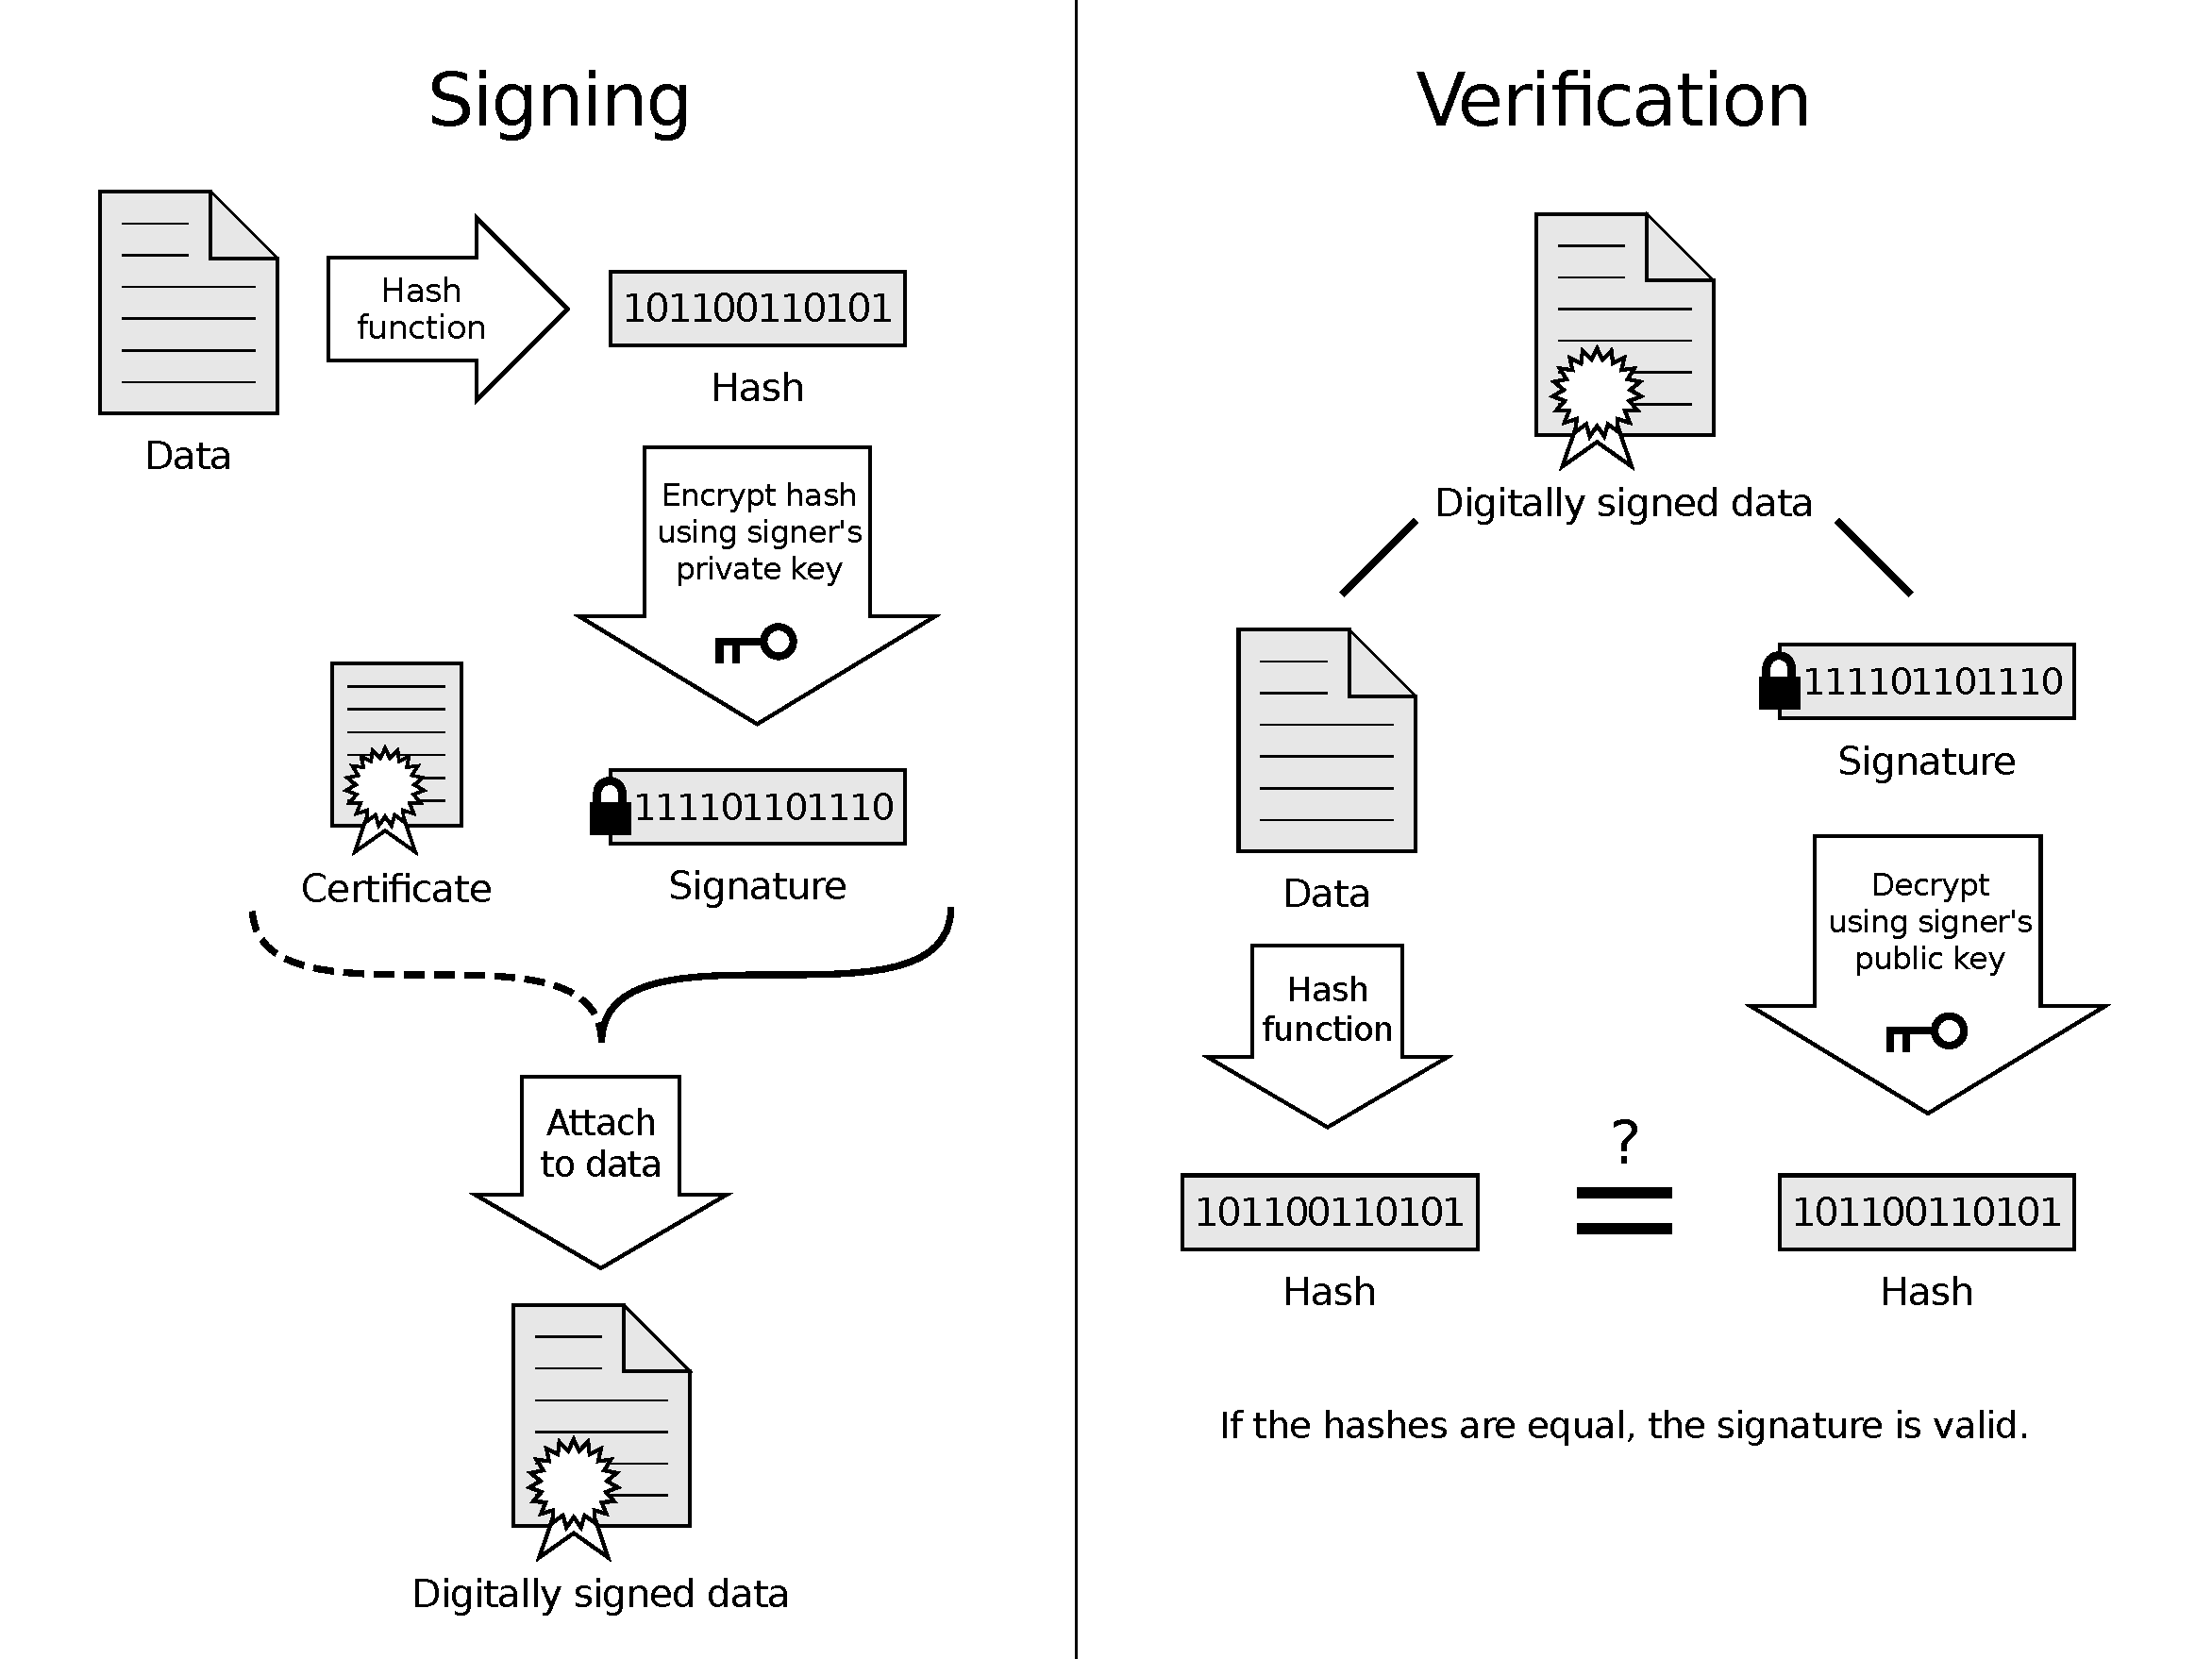
\includegraphics[width=0.7\textwidth,height=0.7\textheight,keepaspectratio]{figures/digitalsignaturediagram.pdf}
\caption{Diagrama de assinatura digital de documentos (\url{https://commons.wikimedia.org/wiki/File:Digital_Signature_diagram.svg}).}
\label{fig-digi-sign}
\end{figure}

Certificado digital vs. assinatura digital

\vspace{2ex}
O certificado digital é uma documento digital emitido por uma autoridade de certificação (CA). 
As CAs agem como terceiros confiáveis aceitando, autenticando, emitindo e mantendo certificados digitais. 
O certificado digital faz a ligação entre a chave pública e a identidade de um agente, permitindo
verificar se determinada chave pertence a tal pessoa ou entidade.
Modelo de confiança centralizado (PKI, \textit{public key infrastructure}).

\vspace{2ex}
Uma alternativa às CAs é a rede de confiança (\textit{Web of trust}), um modelo de confiança descentralizado.
Utilizado no PGP (\textit{Pretty Good Privacy}).

\end{frame}



\subsection{PGP}
\begin{frame}[allowframebreaks,fragile]
\frametitle{Exemplos PGP}

\begin{lstlisting}[language=bash, label=lst-pgp-ex01, caption={Assinar um documento.}, postbreak=\mbox{$\hookrightarrow$\space}, basicstyle=\fontsize{8}{10}\selectfont\ttfamily]
$ echo "pois só a justa medida do tempo dá a justa natureza das coisas, não bebendo do vinho quem esvazia num só gole a taça cheia" > RaduanNassar.txt
$ gpg --clear-sign RaduanNassar.txt 
$ cat RaduanNassar.txt.asc
-----BEGIN PGP SIGNED MESSAGE-----
Hash: SHA512

pois só a justa medida do tempo dá a justa natureza das coisas, não bebendo do vinho quem esvazia num só gole a taça cheia
-----BEGIN PGP SIGNATURE-----

iQEzBAEBCgAdFiEEp4rIXACghPaEmi4sB7Zpi0fJbb8FAmFN9/oACgkQB7Zpi0fJ
bb/JZAf/UJXiKFayugMYewIfWapVvqHmt3Uu30H8ro2Aj1TVZKm37LLudGwsDGH5
HcqRZtb1pkugVCGZ8tZxg3WTuiYUaPsWBdiich9hQE5CkFasl2SYoAeX8Gn4RhVK
qX60Dfvw3Wm1HgayBfuqjDjxz7TXcpJHF6jte/Ni7kKLB4emgcuCGg17Hw9iOvYl
2RprL8qn7H7V/VuhWH9UG8fXvlDxQHm/yR++Q0lCjhNmT8yTKJsaTqtOfu5frQJv
otQtqfYQ+Wg3pQe/3/BWUW+8cEF8vwV3nRADiScFIwASEYMQ29ozQiCGu8H4FeBn
Ht/L75hqf44yePysO+HG+c+40RX8GQ==
=SSvI
-----END PGP SIGNATURE-----
\end{lstlisting}


\begin{lstlisting}[language=bash, label=lst-pgp-ex02, caption={Verificar a assinatura de um documento.}, postbreak=\mbox{$\hookrightarrow$\space}, basicstyle=\fontsize{8}{10}\selectfont\ttfamily]
$ gpg --verify RaduanNassar.txt.asc
gpg: Signature made sex 24 set 2021 13:08:26 -03
gpg:                using RSA key A78AC85C00A084F6849A2E2C07B6698B47C96DBF
gpg: Good signature from "Leonardo Carneiro de Araujo <leolca@gmail.com>" [ultimate]
gpg: WARNING: not a detached signature; file 'RaduanNassar.txt' was NOT verified!
\end{lstlisting}


\begin{lstlisting}[language=bash, label=lst-pgp-ex03, caption={Assinar um documento e verificar.}, postbreak=\mbox{$\hookrightarrow$\space}, basicstyle=\fontsize{8}{10}\selectfont\ttfamily]
$ gpg --sign RaduanNassar.txt
$ gpg --verify RaduanNassar.txt.gpg
gpg: Signature made sex 24 set 2021 13:20:53 -03
gpg:                using RSA key A78AC85C00A084F6849A2E2C07B6698B47C96DBF
gpg: Good signature from "Leonardo Carneiro de Araujo <leolca@gmail.com>" [ultimate]
\end{lstlisting}


\framebreak 
\begin{lstlisting}[language=bash, label=lst-pgp-ex04, caption={Encriptar um arquivo.}, postbreak=\mbox{$\hookrightarrow$\space}, basicstyle=\fontsize{8}{10}\selectfont\ttfamily]
# encriptando um arquivo 
$ gpg --recipient leolca --encrypt RaduanNassar.txt
$ ls RaduanNassar.txt.gpg
$ gpg --decrypt RaduanNassar.txt.gpg
\end{lstlisting}

\framebreak 
\begin{lstlisting}[language=bash, label=lst-pgp-ex05, caption={Enviando a chave para um servidor de chaves.}, postbreak=\mbox{$\hookrightarrow$\space}, basicstyle=\fontsize{8}{10}\selectfont\ttfamily]
$ gpg --fingerprint leolca@gmail.com
pub   rsa2048 2013-07-08 [SC]
      A78A C85C 00A0 84F6 849A  2E2C 07B6 698B 47C9 6DBF
      uid           [ultimate] Leonardo Carneiro de Araujo <leolca@gmail.com>
      sub   rsa2048 2013-07-08 [E]

$ gpg --keyserver hkp://keyserver.ubuntu.com:80 --send-keys 47C96DBF
gpg: sending key 07B6698B47C96DBF to hkp://keyserver.ubuntu.com:80
\end{lstlisting}

\end{frame}



\subsection{Números aleatórios}
\begin{frame}[allowframebreaks,fragile]
  \frametitle{Números aleatórios}

        \begin{figure}[h!]
        \centering
        \includegraphics[width=0.75\textwidth,height=0.5\textheight,keepaspectratio]{/home/leoca/ee/ufsj/aulas/ti/images/dilbert.png}
        %\caption{Df.}
        \label{fig:dilbert-random}
        \end{figure}

  \begin{itemize}
  \item ``Anyone who attempts to generate random numbers by deterministic means is,
          of course, living in a state of sin''. (John von Neumann)
  \item ``randomness is in the eye of the beholder'' (Numerical Recipes)
  \end{itemize}

  As três fontes de aleatoriedade:
  \begin{itemize}
  \item aleatoriedade do ambiente
  \item aleatoriedade nas condições iniciais
  \item geração intrínseca de aleatoriedade
  \end{itemize}

  \begin{quote}
  ``assuming that there is a random external environment which
    continually affects the system one is looking at, and continually
    injects randomness into it.''

    (...)

  ``the basic mechanisms responsible for phenomena that we see in nature are
    somehow the same as those responsible for phenomena that we see
    in simple programs''.

    (...)

  ``simple programs can produce apparently random behavior even when they are given no random input whatsoever''.

  (Stephen Wolfram, A New Kind of Science)
  \end{quote}

  \begin{figure}[h!]
  \centering
  \includegraphics[width=0.75\textwidth,height=0.5\textheight,keepaspectratio]{/home/leoca/ee/ufsj/aulas/programming/random/nkspg299.png}
  \caption{Três mecanismos que podem ser responsáveis pela aleatoriedade: ambiente, condição inicial e
          geração intrínseca (Stephen Wolfram, A New Kind of Science).}
  \label{fig:nkspg299}
  \end{figure}

  \framebreak

  \begin{figure}[h!]
  \centering
  \includegraphics[width=0.75\textwidth,height=0.7\textheight,keepaspectratio]{/home/leoca/ee/ufsj/aulas/programming/random/nkspg27.png}
  \caption{Regra 30 - automato celular (Stephen Wolfram, A New Kind of Science).}
  \label{fig:nkspg27}
  \end{figure}

  \framebreak

  \begin{quote}
  ``I believe that this mechanism [intrinsic randomness] is in fact ultimately
    responsible for a large fraction, if not essentially all, of the
    randomness that we see in the natural world. (...) to get randomness
    in a particular system it turns out that there is no need for continual
    interaction between the system and an external random environment''.
    (Stephen Wolfram, A New Kind of Science)
  \end{quote}

  \framebreak

  Números Aleatórios gerados computacionalmente.

  O seguinte método é utilizado desde o final dos anos 1940 em diversos sistemas computacionais:
  \begin{quote}
  ``if one successively multiplies a number by various constant factors,
    and then looks at the digit sequences of the numbers that result (...)
    the patterns of digits obtained in this way seem quite random. (...)
    For practical reasons, such generators typically keep only, say, the
    rightmost 31 digits in the numbers at each step.'' (Stephen Wolfram,
    A New Kind of Science)
  \end{quote}

  \framebreak 
  \begin{figure}[h!]
  \centering
  \includegraphics[width=0.8\textwidth,height=0.8\textheight,keepaspectratio]{/home/leoca/ee/ufsj/aulas/programming/random/nkspg319.png}
  %\caption{.}
  \label{fig:nkspg319}
  \end{figure}

  \framebreak
  \begin{figure}[h!]
  \centering
  \includegraphics[width=0.8\textwidth,height=0.8\textheight,keepaspectratio]{/home/leoca/ee/ufsj/aulas/programming/random/nkspg320a.png}
  %\caption{.}
  \label{fig:nkspg320a}
  \end{figure}

  \framebreak
  \begin{figure}[h!]
  \centering
  \includegraphics[width=0.8\textwidth,height=0.8\textheight,keepaspectratio]{/home/leoca/ee/ufsj/aulas/programming/random/nkspg320b.png}
  %\caption{.}
  \label{fig:nkspg320b}
  \end{figure}

  \framebreak
  \begin{figure}[h!]
  \centering
  \includegraphics[width=0.8\textwidth,height=0.8\textheight,keepaspectratio]{/home/leoca/ee/ufsj/aulas/programming/random/nkspg320c.png}
  %\caption{.}
  \label{fig:nkspg320c}
  \end{figure}


  \framebreak
  \lstinputlisting[language=Matlab,basicstyle=\footnotesize]{/home/leoca/ee/ufsj/aulas/ti/hw/simulations/rndnumberexample2.m}

  \framebreak
  Gerador de número aleatório Lehmer:
  \begin{equation}
  X_{k+1} = g \cdot X_k \mod n
  \end{equation}
  onde $n$ é um número primo ou uma potência de um número primo,
  o multiplicador $g$ é uma raiz primitiva módulo $n$ e a semente
  $X_0$ é co-primo com $n$.

  \url{https://en.wikipedia.org/wiki/Lehmer_random_number_generator}

  \framebreak
  \lstinputlisting[language=Matlab,postbreak=\mbox{$\hookrightarrow$\space}, basicstyle=\fontsize{8}{10}\selectfont\ttfamily]{/home/leoca/ee/ufsj/aulas/programming/tarefas/prandom/randomnumbergenerator.m}

  \framebreak
  Números aleatórios em Linux

  \lstinputlisting[language=bash,postbreak=\mbox{$\hookrightarrow$\space}, basicstyle=\fontsize{8}{10}\selectfont\ttfamily]{/home/leoca/ee/ufsj/aulas/ti/hw/simulations/rndlinuxex.txt}

\end{frame}








\subsection{Hash}
\begin{frame}[allowframebreaks,fragile]
  \frametitle{Hash}

Uma função hash é uma função de mapeamento de dados de tamanho qualquer 
em dados com tamanho fixo.

  \begin{figure}[h!]
  \centering
  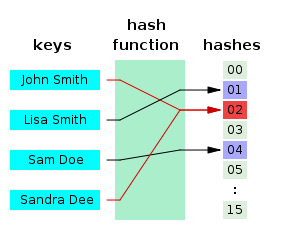
\includegraphics[width=0.33\textwidth,height=0.7\textheight,keepaspectratio]{figures/hashkeys.png}
  \caption{Mapeamento.}
  \label{fig:hashkeys}
  \end{figure}

\framebreak

Alguns exemplos de utilização:
\begin{itemize}
\item Hash Tables
\item Cache (grande quantidade de dados armazenados em media lenta)
\item Bloom filters (estrutura de dados probabilística usada para testar se um elemento pertence a um conjunto)
\item Encontrar duplicidades ou similaridades (exemplo: banco de dados, sequência de DNA)
\item Proteger e autenticar dados 
\end{itemize}

\framebreak

Tempo de Acesso
\begin{itemize}
\item lista simples $O(n)$
\item árvore binária balanceada $O(\log n)$
\item hash tables $O(1)$
\end{itemize}

Usar \emph{hash table} fará com que todas operações (adição, remoção, verificação) tenham custo $O(1)$.
No pior caso (colisão de todas as chaves) a performance será $O(n)$, igual à performance
de uma lista encadeada (se utilizarmos lista para solucionar colisão). 
Podemos usar uma árvore balanceada para nos casos de colisão e assim garantir 
que a pior performance será $O(\log n)$.

\framebreak

Propriedades de um função hash:
\begin{description}
\item[Determinística] -- para um determinado dado de entrada a saída produzida será sempre a mesma saída
\item[Uniformidade] -- os valores de hash devem ser gerados com a mesma probabilidade, uniformemente distribuídos. 
Em aplicações onde queremos a busca de similaridade podemos abrir mão da uniformidade para obter continuidade,
de forma que sequências de dados similares sejam mapeadas em valores iguais ou quase iguais
\item[Não Inversível] -- para aplicações criptográficas isto é um requisito
\item[Extensão pré-definida] -- estes valores podem ser utilizados para indexar um array. 
Funções de hash criptográfico utilizam valores de hash grandes para assegurar a complexidade
da inversão por força bruta, SHA-1, por exemplo, utiliza valores de 160-bits.
Funções de hash dinâmica possuem extensão variável.
\item[Difusão] -- para $k_1 \neq k_2$, conhecer $h(k_1)$ não deve fornecer nenhuma informação sobre $h(k_2)$,
por exemplo, se $k_1$ e $k_2$ diferem em apenas 1 bit, então todos os bits de $h(k_2)$ devem diferir
de $h(k_1)$ com probabilidade $1/2$.
\end{description}

\framebreak

  \begin{figure}[h!]
  \centering
  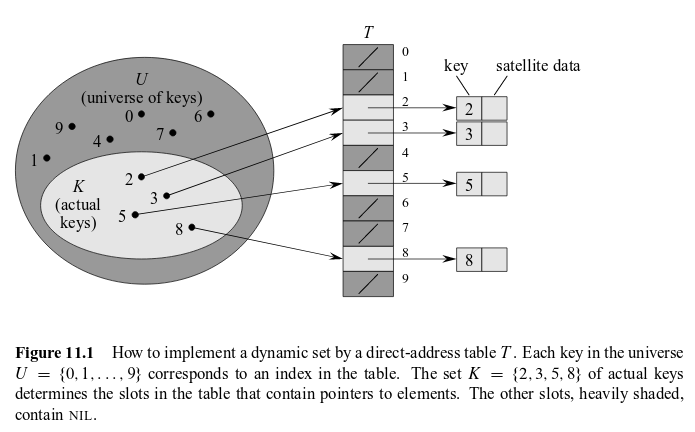
\includegraphics[width=0.8\textwidth,height=0.7\textheight,keepaspectratio]{figures/hash-fig111.png}
  \caption{Hash.}
  \label{fig:hash-fig111}
  \end{figure}

\framebreak

  \begin{figure}[h!]
  \centering
  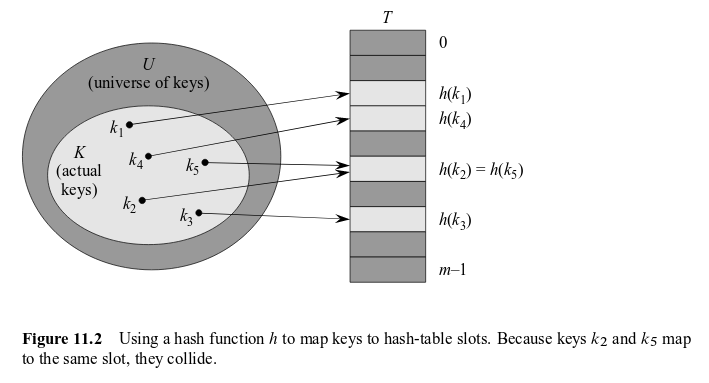
\includegraphics[width=0.8\textwidth,height=0.7\textheight,keepaspectratio]{figures/hash-fig112.png}
  \caption{Hash - colisão.}
  \label{fig:hash-fig112}
  \end{figure}

\framebreak

  \begin{figure}[h!]
  \centering
  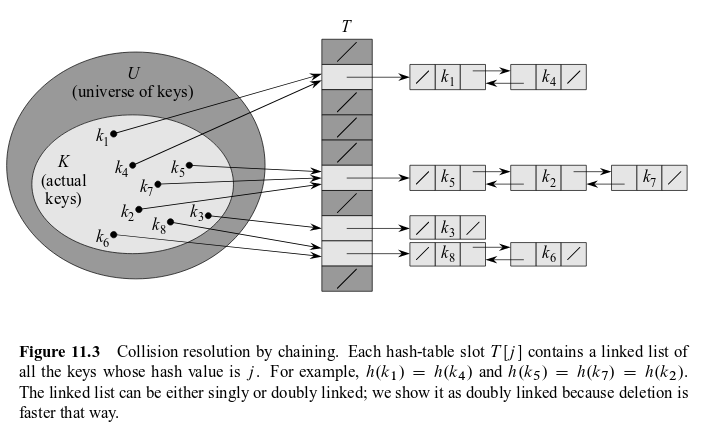
\includegraphics[width=0.8\textwidth,height=0.7\textheight,keepaspectratio]{figures/hash-fig113.png}
  \caption{Hash - encadeamento.}
  \label{fig:hash-fig113}
  \end{figure}

\framebreak

Funções de Hash
\begin{description}
\item[Função de Hash trivial] -- Quando o universo dos dados é pequeno, podemos interpretar os próprios dados como inteiros, sendo
eles mesmo o valor hash de si próprios.
\item[Função de Hash perfeita] -- É uma função injetiva, não gerando colisões.
\item[Função de Hash mínima perfeita] -- Uma função para $n$ chaves é mínima quando sua extensão consiste em inteiros consecutivos de $0$ a $n-1$
sem deixar buracos, gerando assim uma tabela hash compacta.
\end{description}

\framebreak

Função de Hash Modular
 $$h(k) = k \mod m$$

\begin{itemize}
\item $m$ não deve ser uma potência de 2
\item tipicamente escolhemos $m$ primo
  (um primo que não esteja muito próximo de uma potência de 2)
\item a extensão de $h$ será $m$
\item em geral, não garante uniformidade, podendo levar a muitas colisões
\end{itemize}


\framebreak

Para uma chave inteiro, podemos fazer:
\begin{lstlisting}[language=C, label=lst-hash-mod, caption={Função de Hash Modular.}, postbreak=\mbox{$\hookrightarrow$\space}, basicstyle=\fontsize{8}{10}\selectfont\ttfamily]
int hash(int key) {
    return key % M;
}
\end{lstlisting}


No caso de strings, faremos:
\begin{lstlisting}[language=C, label=lst-hash-mod, caption={Função de Hash Modular.}, postbreak=\mbox{$\hookrightarrow$\space}, basicstyle=\fontsize{8}{10}\selectfont\ttfamily]
int h = 0;
for (int i = 0; i < s.length(); i++)
    h = (31 * h + s(i)) % M;
\end{lstlisting}

\framebreak

Método multiplicativo

  $$h(k) = \lfloor m (kA \mod 1) \rfloor $$

Note que $kA \mod 1$ representar a parte fracionária de $kA$.
O valor escolhido para $m$ não é crítico.
Tipicamente escolhemos $m$ como uma potência de 2 ($m=2^p$, para algum inteiro $p$).


\framebreak

\begin{lstlisting}[language=bash, label=lst-hash-ex01, caption={Hash de arquivo.}, postbreak=\mbox{$\hookrightarrow$\space}, basicstyle=\fontsize{8}{10}\selectfont\ttfamily]
$ md5sum RaduanNassar.txt
f6955a7644083fb61d6ea97578e2727a  RaduanNassar.txt

$ sha256sum RaduanNassar.txt
e98f57d7d3e3887503ce69a7bd6df4a6c8a8dc59455ad1e20f435683000ee3c9  RaduanNassar.txt

$ sha256sum RaduanNassar.txt | sha256sum --check
RaduanNassar.txt: OK
\end{lstlisting}

\framebreak
Sugestões de leitura:
\vspace{2ex}

\fullcite{cormen2009}
\vspace{2ex}

\url{https://algs4.cs.princeton.edu/34hash/}
\vspace{2ex}

\url{http://www.cs.cornell.edu/courses/cs312/2008sp/lectures/lec20.html}
\vspace{2ex}

\url{https://www.ime.usp.br/~pf/estruturas-de-dados/aulas/st-hash.html}
\vspace{2ex}

\url{https://en.wikipedia.org/wiki/Hash_function}




\end{frame}
